% Diese Zeile bitte -nicht- aendern.
\documentclass[course=erap]{aspdoc}
\usepackage[utf8]{inputenc}
\usepackage[T1]{fontenc}
\usepackage{amsmath}
\usepackage{hyperref}
\usepackage{float}
\usepackage{graphicx}
\usepackage[numbers,sort&compress]{natbib}

%%%%%%%%%%%%%%%%%%%%%%%%%%%%%%%%%
%% TODO: Ersetzen Sie in den folgenden Zeilen die entsprechenden -Texte-
%% mit den richtigen Werten.
\newcommand{\theGroup}{276} % Beispiel: 42
\newcommand{\theNumber}{A505} % Beispiel: A123
\author{Awar Satar \and Yiyang Xie \and Jingjing Yu}
\date{Sommersemester 2023} % Beispiel: Wintersemester 2019/20
%%%%%%%%%%%%%%%%%%%%%%%%%%%%%%%%%

% Diese Zeile bitte -nicht- aendern.
\title{Gruppe \theGroup{} -- Abgabe zu Aufgabe \theNumber}

\begin{document}
\maketitle

\section{Einleitung}
Im digitalen Zeitalter sind die Sicherheit und die Integrität von Daten von großer
Bedeutung.
Kryptographische Hashfunktionen spielen eine entscheidende Rolle in
diesem Bereich und sind weitreichend in verschiedenen Domänen eingesetzt.
Der
Fokus dieser Arbeit liegt auf dem MD2 Hashing Algorithmus, welcher im RFC 1319
der Internet Engineering Task Force (IETF) beschrieben ist~\cite{rfc1319}.
\\
Obwohl der MD2 Algorithmus mittlerweile als obsolet gilt, bietet er einen
interessanten Ansatz zur Untersuchung der Grundlagen und der Entwicklung
kryptographischer Hashfunktionen.
\\
Die zu verarbeitenden Daten in solchen Hashing Algorithmen müssen stets ein
Vielfaches der Blocklänge sein, was durch Padding erreicht wird.
Eines der
Verfahren, das diese Anforderung erfüllt, ist das PKCS\#7~\cite{rfc2315}.
\\
Die erste Aufgabe besteht darin, dieses Verfahren genauer zu erforschen und in
dieser Arbeit zu beschreiben.
\\
Darüber hinaus gilt es, die genaue Funktionsweise der Berechnung von Prüfsumme
und Hashwert zu erläutern.
Insbesondere wird in beiden Schritten eine Substitutionsbox verwendet, deren
Werte es zu klären gilt.
\\
Letztendlich werden wir die Angriffe auf den MD2-Algorithmus sowie die Alternativen,
die heute verwendet werden, diskutieren.
Dadurch werden die Gründe für das Auslaufen des MD2 und die Fortschritte in der
Kryptographie verdeutlicht.


\section{Lösungsansatz}
\subsection{Kryptographischer Hintergrund}
\label{sec:crypto}

Eine kryptographische Hashfunktion, auch \glqq Message Digest\grqq -Funktion genannt ist
eine Familie von Hashing Algorithmen
, die eine Nachricht $m$ auf einen \glqq Digest\grqq $\ h(m)$ reduzieren.
Die Idee ist also
eine Nachricht durch Hashing kompakt zu repräsentieren, was bspw.
für Signaturen
von langen Texten Anwendung findet~\cite{menezes2018} und \
da beim Hashing  das Urbild der Funktion in der Mächtigkeit die Ergebnismenge deutlich
übersteigt, ist es allerdings möglich sogenannte Kollisionen zu finden, also ein
$m_k \ne m$ mit $h(m) = h(m_k)$.
Für kryptographische Hashfunktionen wurden
entsprechend Eigenschaften festgelegt, die aus einer Sicherheitsperspektive
erstrebenswert sind:\cite{kryptografischeHashfunktion}

\begin{itemize}
      \item [(1)] $\forall m:  H(m)$ ist einfach zu berechnen.
      \item [(2)] \textbf{Urbildresistenz:} Für ein gegebenes $h = H(m)$ ist das Bestimmen des
            Wertes $m$ mit $m = H^{-1}(h)$ nicht effizient möglich, d.h.\ es ist nicht effizient
            möglich mittels $H(m)$ auf $m$ zu schließen.
      \item [(3)] \textbf{schwache Kollisionsresistenz:} Es ist nicht effizient möglich zu einem
            gegebenem $m$ ein $m'$ zu finden, sodass $H(m) = H(m')$.
      \item [(4)] \textbf{starke Kollisionsresistenz:} Es ist nicht effizient möglich ein
            beliebiges Paar $(m, m')$ zu finden, sodass $H(m) = H(m')$.
\end{itemize}

MD2 Hashing besteht aus 3 Schritten. Zuerst wird die Nachricht auf ein
Vielfaches von 16 Byte ergänzt. Anschließend wird eine Prüfsumme berechnet und 
an das Ende der Nachricht angehängt. Zum Schluss wird die Nachricht in 18 
Durchläufen komprimiert oder gehasht. 
Wir werden auf jeden dieser Schritte im Detail eingehen. 

\subsection{PKCS\#7 Padding: Implementierung und Optimierung}

In der kryptographischen Welt ist das Padding von Nachrichten eine weit verbreitete
Technik, um die Größe der zu verarbeitenden Daten auf ein Vielfaches der Blocklänge
zu bringen.
Ein gängiges Verfahren dafür ist das PKCS\#7 Padding, das hier genauer
erörtert wird.
Es handelt sich um ein standardisiertes Verfahren, das in RFC 2315
ausführlich beschrieben wird~\cite{rfc2315}.
\\
Die grundlegende Idee des PKCS\#7 Paddings besteht darin, den fehlenden Platz in
einem Block mit einer Sequenz von Bytes zu füllen, deren Wert der Länge der
Sequenz entspricht.
Bei einer Blocklänge von 16 Bytes kann also jeder Block,
unabhängig von seiner ursprünglichen Größe, auf die erforderliche Länge gebracht werden.
\\
Eine Optimierungsstufe kann durch den Einsatz von SIMD-Instruktionen erreicht
werden, wie in der Funktion \texttt{padding\_opt\_V0} gezeigt.
Durch die Verwendung
der SIMD-Instruktion \texttt{\_mm\_storeu\_si128} können mehrere Bytes gleichzeitig
geschrieben werden, was zu einer deutlich verbesserten Leistung führt.
\\
Insgesamt ermöglichen diese Optimierungen eine effizientere Anwendung des PKCS\#7
Paddings, was in vielen kryptographischen Kontexten von großem Nutzen sein kann.

\subsection{Berechnung der Prüfsumme}

Die Berechnung der Prüfsumme und des Hashwerts sind zentrale Bestandteile des
MD2-Algorithmus. Ohne dem Prüfsummen-Byte ist der MD2 unsicher \cite{rogier1997}.
In diesem Abschnitt wird die genaue Funktionsweise dieser
Berechnungen erläutert und der Einsatz der Substitutionsbox (S-Box) in diesen
Prozessen verdeutlicht.
Die S-Box, die in diesen Berechnungen verwendet wird, ist ein wesentliches
Element.
Es handelt sich um ein festes, vordefiniertes Array von 256 Werten,
das für die Substitution der Eingabewerte verwendet wird.
Die Werte in der S-Box
sind so gewählt, dass sie den kryptographischen Sicherheitsanforderungen genügen
und das Ausgabebild stark verändern, selbst wenn nur kleine Änderungen an der
Eingabe vorgenommen werden (Diffusion).
Die Prüfsumme wird erstellt, indem eine Checksummen-Funktion auf die Nachricht
angewendet wird, wobei jedes Byte der Nachricht in 16 Byte Blöcken verarbeitet wird.
Das aktuelle Byte des Blocks nennen wir von nun $b_i$ und das 16 Byte Array der
Checksumme $s$.
Ein laufender Totalisator $l$ beginnt am Anfang der Funktion zunächst bei Null $c = 0$.
Anschließend wird der  Index des nächsten Wertes aus der Substitutionsbox mit
$t = b_i \oplus l$ berechnet.
Die Prüfsumme wird an dem Index $i$ dann auf $s_i \oplus t$ gesetzt und letztlich
der Totalisator mit $l = s_i$ aktualisiert.
\\
Die S-Box oder S-Tabelle wird in RFC 1319 \cite{rfc1319} beschrieben wie folgt:
\begin{quote}
    This step uses a 256-byte "random" permutation constructed from the digits of $\pi$.      
\end{quote}
Wirft man allerdings einen Blick auf die S-Box ist es schwer den Zusammenhang 
zwischen den Werten in der Tabelle und $\pi$ zu erkennen. 
Ron Rivest klärte dies in einer E-Mail an einen Forennutzer auf. Zur 
Generierung der S-Box wird $\pi$ als Psuedozufallsgenerator verwendet und mittels 
einer modifizierten Form des Durstenfeld-Shuffles wird eine gleichmäßige Verteilung der
Zufallszahlen in der S-Box ermöglicht.\cite{crypto_stackexchange_18444}

\begin{figure}[h]
      \centering
      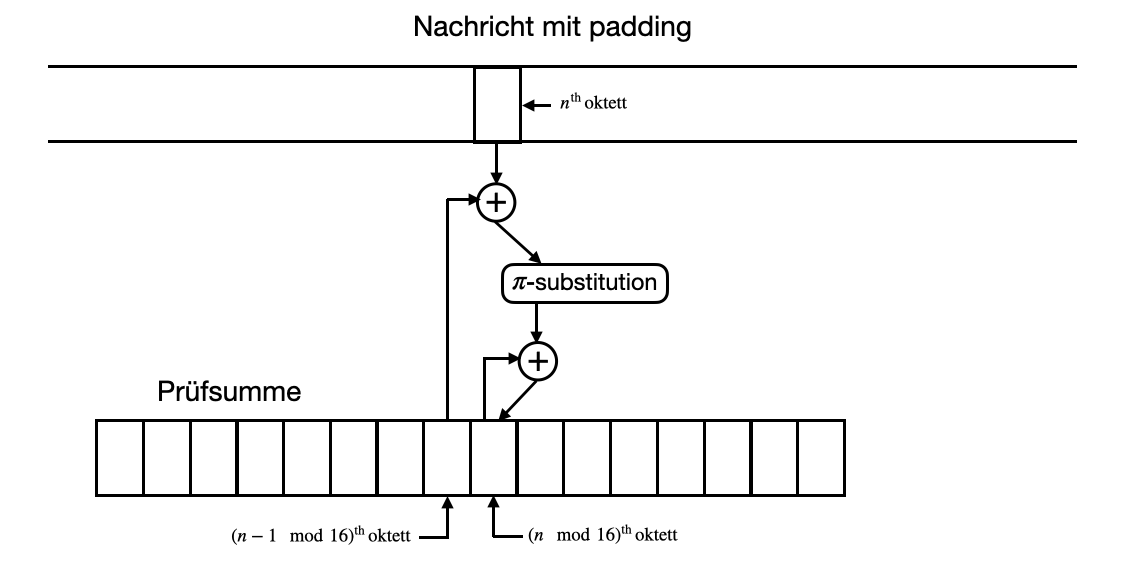
\includegraphics[scale=0.6]{pics/md2diagramchecksum.jpg}
      \caption{Darstellung zur Berechnung der Prüfsumme von MD2\cite{jain2009}}
\end{figure}

Diese genaue Berechnungsmethode, kombiniert mit der Verwendung der S-Box,
trägt zur Sicherheit und Unveränderlichkeit der MD2-Hashfunktion bei.

\subsection{Kompressionsfunktion}


Bei der Kompressionsfunktion handelt es sich um einen iterativen Prozess, bei dem 
mehrere Berechnungsschritte ausgeführt werden, die schließlich zu einem 128-Bit-Hashwert 
führen. Zunächst wird der zu verarbeitende Nachrichtenpuffer in Blöcke von 16 
Bytes aufgeteilt und diese sequenziell verarbeitet. Jeder Block wird in das 
interne Speicher-Array kopiert, das insgesamt 48 Bytes aufnehmen kann und in drei 
Segmente von je 16 Bytes unterteilt ist. Es ist hervorzuheben, dass die ersten 
beiden Segmente vor der Verarbeitung jedes Blocks bereits Daten enthalten können, 
die aus vorherigen Durchläufen stammen. Anschließend wird eine XOR-Operation 
(exklusives Oder) auf den ersten und zweiten Segment des internen Arrays angewendet 
und das Ergebnis in das dritte Segment gespeichert. Das Ergebnis dieser Operation 
fügt eine weitere Ebene der Durchmischung der Daten hinzu und erhöht so die Diffusion 
der Hash-Funktion. Darauf folgen 18 Runden von Substitution und Permutation, die 
auf das gesamte interne Array angewendet werden. In jeder Runde wird jedes Byte 
des internen Arrays durch einen Wert aus der S-Box ersetzt, wobei der Ersatzwert 
durch eine XOR-Operation mit einem temporären Wert bestimmt wird. Nach jeder 
Substitution wird der temporäre Wert aktualisiert, um den nächsten S-Box-Index zu 
bestimmen. Obwohl diese Methode effektiv ist, bietet sie wenig Spielraum für 
Optimierungen. Dies liegt vor allem an der Natur des MD2-Algorithmus, der keine 
Parallelität in seinen Operationen zulässt. Jeder Schritt in der Berechnung ist 
voneinander abhängig und muss in einer strengen Reihenfolge ausgeführt werden. 
Daher sind die Möglichkeiten für Verbesserungen in Bezug auf die Geschwindigkeit 
und Effizienz des Algorithmus begrenzt.

\begin{figure}[h]
      \centering
      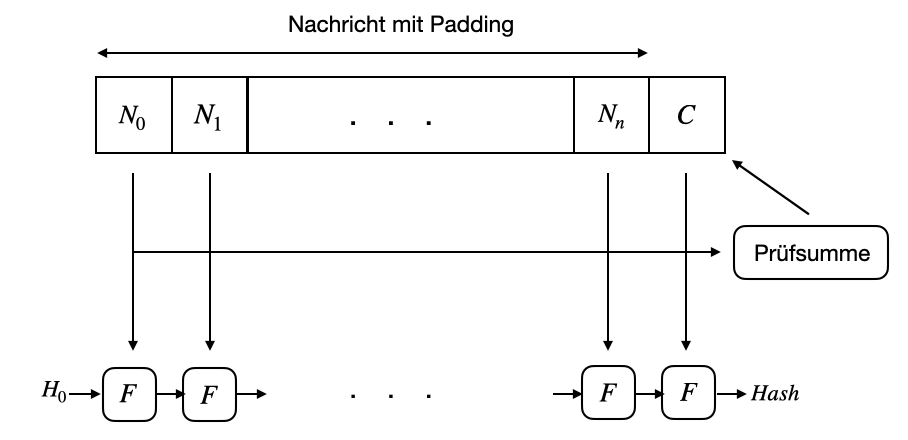
\includegraphics[scale=0.6]{pics/md2.001.jpeg}
      \caption{Berechnung des Hashwertes. $H_0$ beträgt bei MD2 0. 
      Die Darstellung orientiert sich an \cite{knudsen2005}}
\end{figure}


\subsection{Sicherheitsanalyse}

In diesem Abschnitt setzten wir uns konkret mit der kryptographischen Sicherheit 
von MD2 Hashing aus. Hier betrachten wir neben Anwendungsmöglichkeiten auch 
Sicherheitsrisiken und Angriffsvektoren.

\subsubsection{Anwendungsbereiche}
Der MD2-Algorithmus besitzt in der Implementierung eine geringe Komplexität 
und ist zudem schnell berechenbar. Bevor man sicherere Algorithmen entwickelte,
gab es viele Anwedungen für MD2, z.B\@.
\begin{itemize}
      \item \textbf{Überprüfung von Benutzerpasswörtern}
            \\
            Der MD2-Algorithmus kann für die Passwortüberprüfung bei der Benutzeranmeldung
            verwendet werden, indem er vom Klartextabgleich zum Geheimtextabgleich übergeht.
            Hierbei kommt oft auch sog. \glqq Salting \grqq zum Einsatz. Diese Methode 
            wird im Abschnitt \ref{lo:sec_sol} näher behandelt.
      \item \textbf{Überprüfung von Dateiintegrität}
            \\
            Lädt man eine Datei im Internet herunter, kann man oftmals den MD2-Wert 
            der Datei auf der Webseite finden.
            Nachdem der Download abgeschlossen ist, kann der MD2-Wert der heruntergeladenen Datei
            berechnet und mit dem MD2-Wert der Quelle verglichen werden.
            Wenn sie übereinstimmen, ist die Datei vollständig und wurde nicht manipuliert.
            Dadurch kann man die Echtheit der Datei validieren. Natürlich muss 
            hierfür der Hashwert auf der Webseite vertrauenswürdig sein.
     % Leaving this out as this is essentially the same content as the previous point.
      %\item  \textbf{Erkennung von Urheberrechtsverletzung}
      %      \\
      %      Wenn ein Artikel, ein Video oder eine Audiodatei erstellt wird, 
      %      hat sie einen eindeutigen MD2-Wert.
      %      Wenn später eine überarbeitete Version herauskommt, werden die MD2-Werte trotz igleichem
      %      Dateinamen als unterschiedlich eingestuft.
      %      Das Urheberrecht kann anhand des Tags und des MD2-Werts der Datei überprüft werden.
     
\end{itemize}

\subsubsection{Sicherheitslücken}
Von der Verwendung von MD2 Hashing im Internet wird seit 2011 offiziell abgeraten,
doch schon seit 2004 wurde MD2 weitesgehend von MD5 abgelöst. \cite{rfc6149}
Grund dafür sind verschiedene Sicherheitslücken im Algoritmus,
die einen Angriff ermöglichen.
\\
Die Länge des Hashwerts von MD2 beträgt nur 128 bit  bzw $2^{65}$. 
Wegen des Geburtstagsparadoxons sind nur ca. $2^{65/2} = 2^{64}$ Versuche notwendig 
um mit einer Wahrscheinlichkeit von mehr als 50\% eine Kollision zu finden.
Diese relativ kleine Anzahl an Versuchen ist heutzutage effizient leistbar. 
Folglich sind auch komplexere Kollisionsangriffe auf MD2 nicht nötig, da die rohe 
Rechenleistung von heutigen Supercomputern genügt, um ein Kollisionspaar zu 
finden.\cite{kryptografischeHashfunktion}
\\
Das größere Sicherheitsproblem ist die schwache Urbildresistenz von MD2. Der
französische Informatiker Fr{\'e}d{\'e}ric Muller fand 2004 erstmals eine Möglichkeit 
das Urblid eines Hashwertes in besserer Laufzeit als Bruteforce zu ermitteln.
Seine Methode beruht darauf zuerst verschiedene Urbilder der Kompressionsfunktion zu finden, 
was durch den Initialisierungsvektor $0$ möglich ist und anschließend 
die Prüfsummen abzugleichen um ein korrektes Urbild zu ermitteln. 
Die Zeitkomplexität dieser Methode beträgt ca. $2^{104}$ \cite{knudsen2005}, 
was unter den von NIST vorgeschriebenen 128-bit an Sicherheit liegt.\cite{barker2020}
\\
Diese schwache Urbildresistenz wird in sogenannten Rainbow Tables zu 
Nutze gemacht.\cite{oechslin2003}
Diese berechnen die Hashwerte für verschiedenste Passwortkombinationen vor und 
speichern sie in einer Kette, die zwischen Hashwerten und Passwörtern alterniert. 
Dafür muss natürlich die Hashfunktion bekannt sein und auch eine Reduktionsfunktion,
auf deren Details wir im Rahmen dieser Ausarbeitung nicht weiter eingehen,
auf die Hashwerte angewendet werden um wieder Klartexte zu erhalten. 
Mithilfe dieser vorberechneten Werte, erlaubt man sich einen Zeit-Speicher-Ausgleich.

\subsubsection{Sicherheitsmaßnahmen}

%left out due to space limitation
%Diese Schwachstellen haben verschiedene Verwenbarkeiten. Dies sind nur ein Paar
%Konsequenzen die aus einem Angriff entstehen könnten:

%\begin{itemize}
      %\item  \textbf{verfälschte Anmeldeauthentifizierung}
            %\\
            %Wenn die Authentifizierung ein Vergleich von Hashwerten ist, 
            %kann der Angreifer sich mittels einer Hashkollision anmelden.
            %Hierbei muss er nicht einmal das exakte Passwort des Nutzers finden.
      %\item  \textbf{verfälschte digitale Signaturen}
            %\\
            %Wenn Alice (A) und Bob (B) miteinander kommunizieren, fängt ein
            %Man-in-the-Middle-Angreifer (M) die von A an B gesendete Nachricht ab.
            %Da der MD2-Algorithmus öffentlich ist, kann M den ursprünglichen Hashwert der
            %Nachricht berechnen und dann eine neue Nachricht mit demselben Hashwert erzeugen
            %und an B weiterleiten
            %Bisher kann M die gesamte Kommunikation zwischen A und B überwachen und manipulieren,
            %was für A und B schwierig zu erkennen ist.
            %Somit sind Datenintegrität und Authentizität sind gebrochen.
%\end{itemize}
%
%\subsubsection{Verbesserung der kryptografischen Sicherheit}
\label{lo:sec_sol}
\begin{itemize}
      \item \textbf{Salz zur Hashfunktion hinzufügen}
            \\
            Die Hashfunktion wird zu $hash(salt + str)$. \cite{kryptografischeHashfunktion}
            Da der Salt nicht öffentlich verfügbar ist, wird es für einen Angreifer schwieriger,
            Zeichenketten mit identischen Hashwerten zu konstruieren.
            Hierbei wird vor dem 
            Hashing das Klartextwort um einen zufälligen ASCII
            string ergänzt. Dies führt durch Diffusion zu wesentlich anderen Hashwerten als sonst 
            und schützt das System vor Angriffen durch Rainbow Tables. 
            Zudem müsste ein Angreifen dann neben den Passwörtern auch alle möglichen Salts 
            in einem Brute-Force Angriff beachten.
      \item \textbf{Hash-Kollisionen vermeiden}
            \\
            Die Verwendung von Rehash oder geschlossenem Hashing mit offener Adressierung
            sind wirksame Verfahren zur Vermeidung von Hash-Kollisionen.\cite{hashtabelle}
            Jedoch führen sie zu einem Anstieg der Rechenzeit bzw. des Speicherplatzes.
      \item \textbf{Modernere Hashfunktionen verwenden}
            \\
            Es wird von NIST nicht empfohlen, MD2, MD4, MD5, SHA-1, RIPEMD-Algorithmen zu verwenden,
            um sensible Informationen wie Benutzerpasswörter zu
            sichern. \cite{barker2020}
            SHA-512, SHA-3 oder andere fortschrittlichere Hashfunktionen 
            wären bessere Optionen.
\end{itemize}


% TODO: Je nach Aufgabenstellung einen der Begriffe wählen
% \section{Korrektheit/Genauigkeit}
\section{Korrektheit}
Der MD2 Algorithmus ist deterministisch, berechnet also für gleiche Eingabewerte 
gleiche Hashwerte.
Verschiedene Eingabewerte führen mit Ausnahmen von Kollisionen
zu unterschiedlichen Ausgaben.
\\
Da wir hier mit identischen Ausgaben arbeiten, eignet sich eine Diskussion zu 
Genauigkeit in diesem Abschnitt nicht.

\subsection{Testfälle}
Um die Korrektheit unserer Implementierung zu überprüfen, haben wir eine Reihe von Tests
durchgeführt.
Dabei haben wir die von uns berechneten Hashwerte mit denen verglichen, die von verschiedenen
Online-MD2-Rechnern\cite{hashcalculator} erzeugt wurden.
\\
Eine normale .txt-Textdatei wird ausgewählt und der Inhalt dieser Datei
mit unserer Implementierung gehasht.
Anschließend wird dieselbe Datei auf einem Online-MD2-Rechner hochgeladen und
die beiden Hashwerte miteinander verglichen.
Diese Tests sollen sicherstellen, dass unsere Implementierung den Inhalt der
Textdatei nach MD2
korrekt hasht.

\subsection{Fehleranalyse}
Eine vorläufige Implementierung hat nicht zu den gewünschten Ergebnissen geführt.
Unsere Ergebnisse weichten erheblich von den online generierten Ergebnissen ab.
Ferner generierten verschiedene Online-MD2-Rechner unterschiedliche Hashwerte, 
wobei einige mit unseren übereinstimmten.

\subsubsection{Nicht-Text-Dateien}
MD2 behandelt eine rohe Datei als Texteingabe, was das Hashen anderer Dateitypen 
erlauben sollte.
\\
Wir testeten unsere Implementierung mit verschiedenen Dateiformaten wie .o, 
.pdf, .png, .tar usw.
erneut.
Da aber dann der rohe Inhalt der Datei gehasht wird und nicht nur Text, muss der Inhalt der Datei
mit \texttt{uint\_8* buf} anstelle von \texttt{char* buf} dargestellt werden.
Operationen wie \texttt{buf}$[\texttt{len}] = \backslash\texttt{0;}$ können nun 
ausgelassen werden, da der \texttt{string} Datentyp nicht in Verwendung kommt.
\\
Die Leselänge der Quelldatei wird durch die Erstellung der \texttt{stat}-Variablen $statbuf$
und \texttt{fstat(fileno(file), \&statbuf)} ermittelt \cite{fileIO}.
\\
Nach der Verbesserung aller oben beschriebenen Punkte berechnet unser Algorithmus einen
Hash, der in allen Fällen mit dem Wert des Online-MD2-Rechners übereinstimmt.
Dies bestätigt die Korrektheit unserer Implementierung und erlaubt uns die Performanz 
der Implementierung zu testen.


\section{Performanzanalyse} 
Das verwendete System hat folgende Spezifikationen: Intel(R) Core(TM) i7-10710U
CPU, 1.10 GHz, 16 GB Arbeitsspeicher, Ubuntu 22.04.2 LTS, 64 Bit.
Linux Kernel 5.19.0-45-generic.
Kompiliert wurde mit GCC 11.3.0 mit der Option \texttt{-O2}.
\\
Performance-Tests werden für V0 (die Implementierung mit Vektoroptimierung)
und V1 (die Implementierung mit Wrapper-Funktionen für String-Operationen) durchgeführt.

\subsection{Laufzeit-Tests}
Wir verglichen die Laufzeit für Operationen zwischen Dateien mit unterschiedlichen Datenmengen,
 unterschiedlicher Entropie (Inhaltswiederholung), Datenlängen, die
(nicht) ganzzahlige Vielfache von 16 sind und Dateien mit redundanten 
Datenlängen von 1 oder 15 usw.

\subsubsection{Voraussetzungen für die Laufzeit-Tests}
Wir gestalteten unsere Tests so, dass Sie die in der Vorlesung genannten 
Voraussetzungen \cite{benchmarking} erfüllen: 
\begin{itemize}
    \item Um die Genauigkeit der Ergebnisse zu garantieren, wurde jeder Test 250.000
          Mal wiederholt, so dass die Gesamtlaufzeit 1 Sekunde betrug.
    \item Aufgrund der Varianz der Zeittests führen wird derselben Test
          mindestens dreimal durchgeführt und der Durchschnitt berechnet.
    \item Die Tests wurden auf einem Personal Computer durchgeführt, da stärkere 
         Varianzen beim Testen in der \texttt{lxhalle} über \texttt{ssh} beobachtet wurden. 
    \item Der Computer sollte sich nicht im Energiespar-Modus befinden \cite{energySaving}, sonst
          verlängert sich die Laufzeit und die Varianz der Ergebnisse nimmt zu.
    \item Die Optimierungsstufe sollte mindestens \texttt{-O2} sein. 
    \item Es werden \texttt{clock\_gettime} als funktion und \texttt{CLOCK\_MONOTONIC} als Uhr
          gewählt, da sie präziser sind als andere Funktionen.  
\end{itemize}
  
Die Zeittests erfordern ein sehr hohes Niveau an Genauigkeit und Präzision, \cite{energySaving}
andernfalls sind die Ergebnisse gegenstandslos bzw. unwissenschaftlich.

\subsubsection{Ergebnisse der zeitbasierten Tests}
Der Unterschied in der Laufzeit zwischen $V0$ und $V1$ ist unter \texttt{O2} nicht signifikant,
testet man allerdings in \texttt{O0} ist $V0$ deutlich besser als $V1$.
Aufgrund der Voraussetzungen konzentrieren
wir uns in diesem Abschnitt jedoch auf die Ergebnisse in \texttt{O2}.
Auf Grundlage der Ergebnisse der Laufzeittests und \ref*{img:test1} kommen wir zu folgenden Entschlüssen:
\begin{itemize}
    \item [(a)] \textbf{Die Laufzeit ist proportional zur Dateigröße.}
          \\
          Die verbrauchte Zeit steigt mit steigender Dateigröße linear an.
    \item [(b)] \textbf{Mittels loop-unrolling kann die Laufzeit reduziert werden}\cite{gnuOptimierung}
          \\
          Fügt man die Option \texttt{-funroll-loops} in die Makefile ein, kann man 
          einen klaren Speedup erkennen.

    \item [(c)] \textbf{Kein Zusammenhang zwischen SIMD und verbrauchter Zeit}
          \\
          Im MD2-Hash-Algorithmus umfassen die Berechnung der Prüfsumme und die 
          Generierung des Hash-Wertes mehrere Schritte. Einer dieser Schritte 
          ist die Byte-Substitution, die mehrmals auf dem Eingabe-String durchgeführt wird.
          Dieser Prozess erfolgt sequenziell und behandelt jedes Byte einzeln. 
          Die Substitution basiert sowohl auf dem aktuellen Byte-Wert, der 
          verarbeitet wird, als auch auf dem Ergebnis, das aus dem vorherigen 
          Substitutionsschritt erzielt wurde und ist somit iterativ in der Natur.
          Eine Vektorisierung mittels SIMD oder Multithreading erweist sich deswegen als kaum effektiv.
\end{itemize}

          \begin{figure}[H]
            \label{img:test1}
                  \centering
                  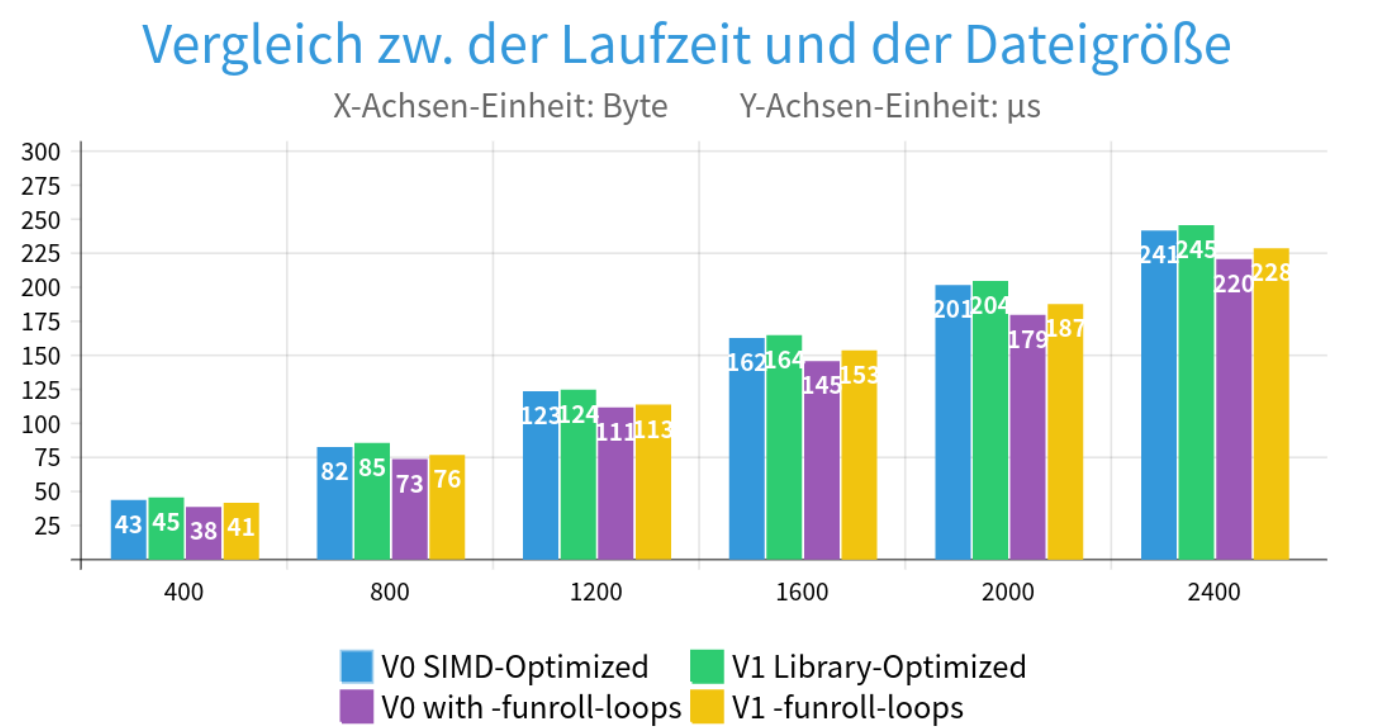
\includegraphics[height=6cm, width=10cm]{pics/4laufzeit.png}
                  \caption{Vergleich zwischen Laufzeit und Dateigröße.
                    Die Berechnungen wurden mit Eingabgrößen von 400 bis 2400 Bytes jeweils 250000 mal
                    durchgeführt und das arithmetische Mittel für jede Eingabegröße auf der $y$ Achse eingetragen.
                    }
              \noindent
          \end{figure}


\subsection{Tests zur Programmgröße}
Bei der Untersuchung Operationenanzahl (Menge des Codes) stellten wir fest,
dass $V0$ deutlich weniger Operationen benötigt als $V1$.
\\
Die .c-Dateien zeigen, dass die Implementierung mit Intrinsics die beste ist.
Darüber hinaus wurde der Assembly-Code der verschiedenen Implementierungen mit dem Terminalbefehl
\texttt{objdump -d -M intel main | less} überprüft. \cite{analyseDesKompiliertenProgramms}.

\begin{figure}[H]
        \centering
        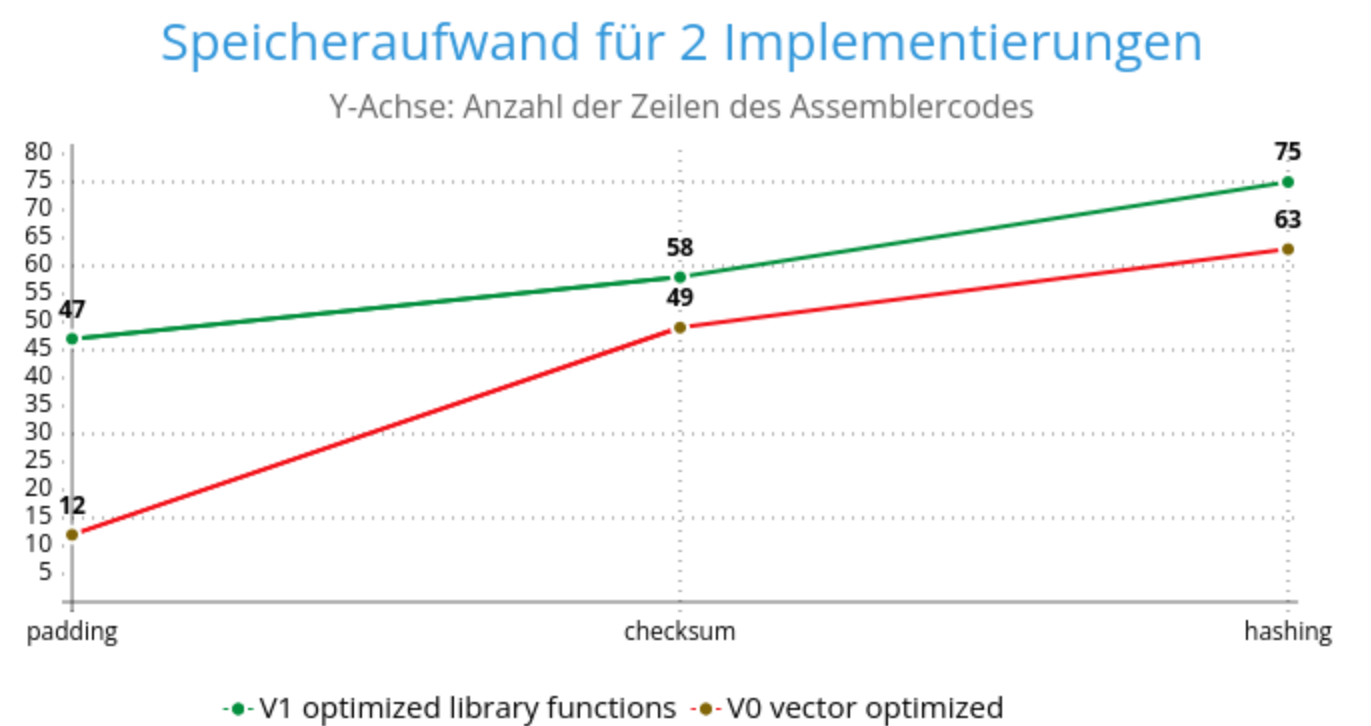
\includegraphics[height=6cm, width=10cm]{pics/SpeicherAufwand.png}
        \caption{Speicheraufwand von $V0$ und $V1$}
        \label{img:test2}
    \noindent
\end{figure}

Der auf V0 basierende Assembly-Code hat viel weniger Vergleichs -und Sprungoperationen.
Außerdem wurde in $V0$ die xmm-Erweiterung eingeführt, welche die Anzahl der Instruktionen
weiter reduziert (vgl. \ref{img:test2}).
\\
Wird die Option \texttt{-funroll-loops} verwendet, wird der entstehende Code
größer und weniger lesbar (vgl. \ref{img:test3}).

\begin{figure}[H]
        \centering
        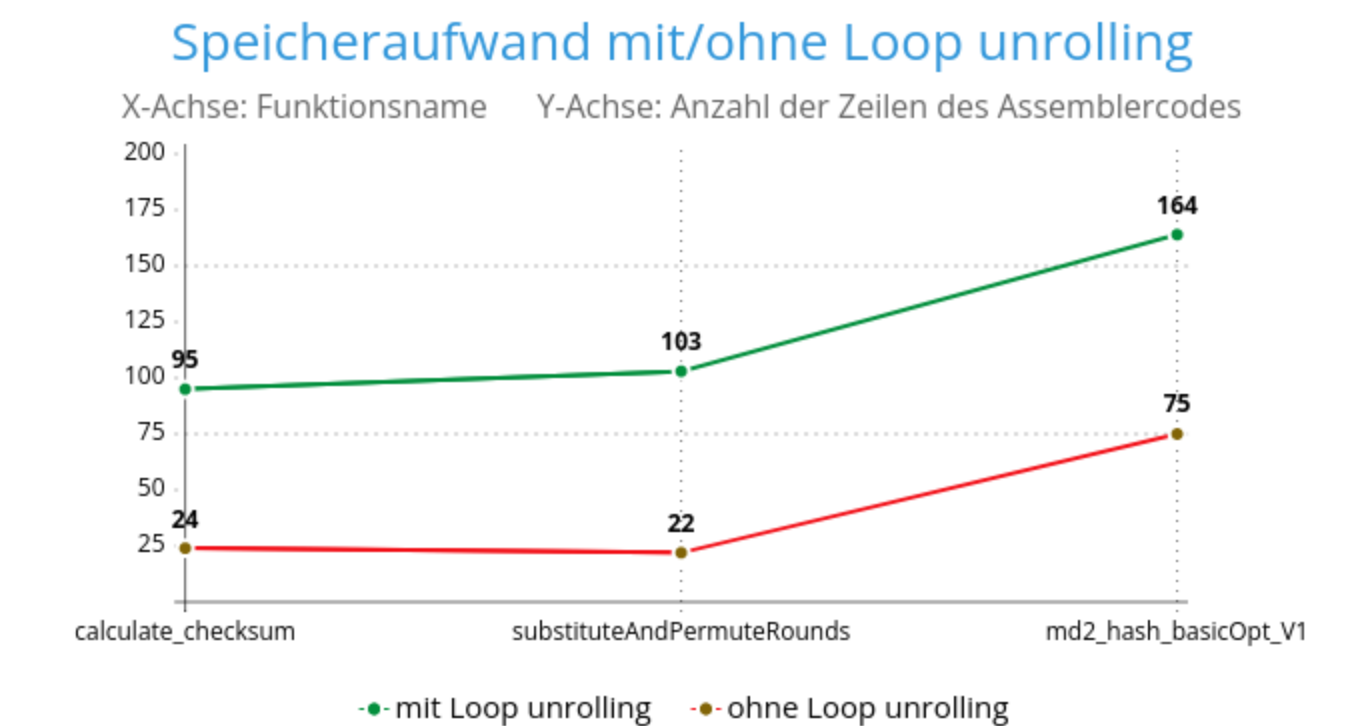
\includegraphics[height=6cm, width=10cm]{pics/loopUnrolling.png}
        \caption{Speicheraufwand mit bzw. ohne Loop unrolling}
        \label{img:test3}
    \noindent
\end{figure}

Loop-Unrolling kann die Laufzeit des Programms reduzieren, kommt aber auf kosten von
Lesbarkeit und die Speicher.

%Lack of detail. Need to elaborate further
%\subsection{Andere Optimierungen}
%Wir nahmen zudem weitere, kleinere Optimierungen an unserer Implementierung vor.
%\\
%Ursprünglich basierte die Logik auf \texttt{if}-Anweisungen oder \text{switch}-Anweisungen.
%\\
%Danach haben wir unsere Codelogik optimiert, um sie weniger redundant zu machen.
%Wie in der Vorlesung erwähnt\cite{gnuOptimierung}, können fortgeschrittenere Algorithmen zur
%Optimierung verwendet werden.
%\\
%Anschließend haben wir die GCC-Wrapper-Funktionen verwendet, um unsere Implementierung
%weiter zu optimieren.
%Darüber hinaus haben wir auch manuelle Schleifenvertauschungen und
%Schleifenerweiterungen ausprobiert.
%\\
%Allerdings zeigten sie nicht den gewünschten Optimierungseffekt oder sogar eine
%Verschlechterung.

\subsection{Zusammenfassung der Performanzanalyse}
Die Implementierung mit Intrinsics ist am effizientesten.
Die Verwendung von Loop Unrolling führt zu einem deutlichen Geschwindigkeitszuwachs,
die Codegröße steigt damit aber auch an.
%\\
%Man könnte sich für weitere Verbesserungen tiefer mit Multithreading auseinandersetzen.
%Die Codegröße dieses Projekts ist nicht groß genug, um eine signifikante Optimierung
%der Laufzeit unter $O2$ zu erreichen, aber aus Sicht der Codegröße schon.
\\
MD2 ist ein byteorientierter Hash-Algorithmus.\cite{rfc1319}
In der Tat verarbeiten alle Instruktionen 8-Bit Blöcke.
Dies verbessert zwar die Kompatibilität mit älteren Architekturen und vereinfacht die
Implementierung, führt aber auch
zu der schlechten Performanz und Optimierbarkeit des MD2-Algorithmus.
\\
Heutige Prozessoren können (mindestens) 32-Bit-Datenwörter verarbeiten, woran sich alle
modernen Hashfunktionen orienteren, z.B. MD4, MD5, die Familien RIPEMD
und SHA.
Daher schränkt die Logik des Algorithmus allein die Optimierungsmöglichkeiten ein.

\goodbreak
\section{Zusammenfassung und Ausblick}
Im Rahmen dieser Arbeit wurde der MD2 Hashing-Algorithmus implementiert und 
auf seine Korrektheit und Performanz auf verschiedenen Limiationen eingegangen.
Auf die Sicherheitsprobleme dieses mittlerweile obsoleten Algorithmus von Ronald Rivest wurde 
ebenfalls eingegangen.
\\
Um dieses Projekt weiterzuführen könnte man weitere Hashfunktionen, die sich etabliert haben,
implementieren und in das Rahmenprogramm einbauen.
Diese erlauben bessere
Optimierungsmöglichkeiten und sind schwerer zu brechen.
Insbesondere die Untersuchung der Auswirkung von Quantum Computing auf jene Hashfunktion
und Laufzeit könnte ein weiteres Projekt bilden.


% TODO: Fuegen Sie Ihre Quellen der Datei Ausarbeitung.bib hinzu
% Referenzieren Sie diese dann mit \cite{}.
% Beispiel: CR2 ist ein Register der x86-Architektur~\cite{intel2017man}.
\bibliographystyle{unsrtnat}
\bibliography{Ausarbeitung}{}

\end{document}
